% !TEX root = ../main.tex

Inicialmente foi necessário entender o problema do qual iriamos tratar, traçar características e definir uma visão com o cliente para impedir problemas futuros como por exemplo problemas de comunicação causados por ambiguidade ou coisas parecidas, estas informações estão esclarecidas no Documento de Visão, presente na sessão \ref{sec:document_de_visao} deste documento.

Após a definição do Documento de Visão iniciou-se a parte de elicitações de requisitos, a modelagem desta está representada na imagem \ref{img:modelagem1}

\begin{figure}[!h]
	\centering
	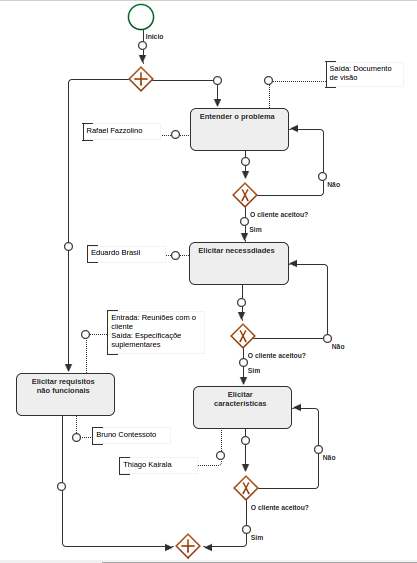
\includegraphics[width=0.8\textwidth]{imgModelagem/modelagem1}
	\caption{Modelagem Parte 1}
	\label{img:modelagem1}
\end{figure}

Após os casos de uso do projeto definidos, vem a parte de definição de prioridades, criação dos \textit{road maps}, assim como detalhamento dos casos de uso e implementação das funcionalidades com maior prioridade do projeto, a modelagem do mesmo esta presente na imagem \ref{img:modelagem2}.

O detalhamento dos casos de uso está presente na sessão \ref{sec:documento_de_caso_de_uso} deste documento, assim como os roads maps se encontram na sessão \ref{sec:road_map}.

\begin{figure}[H]
	\centering
	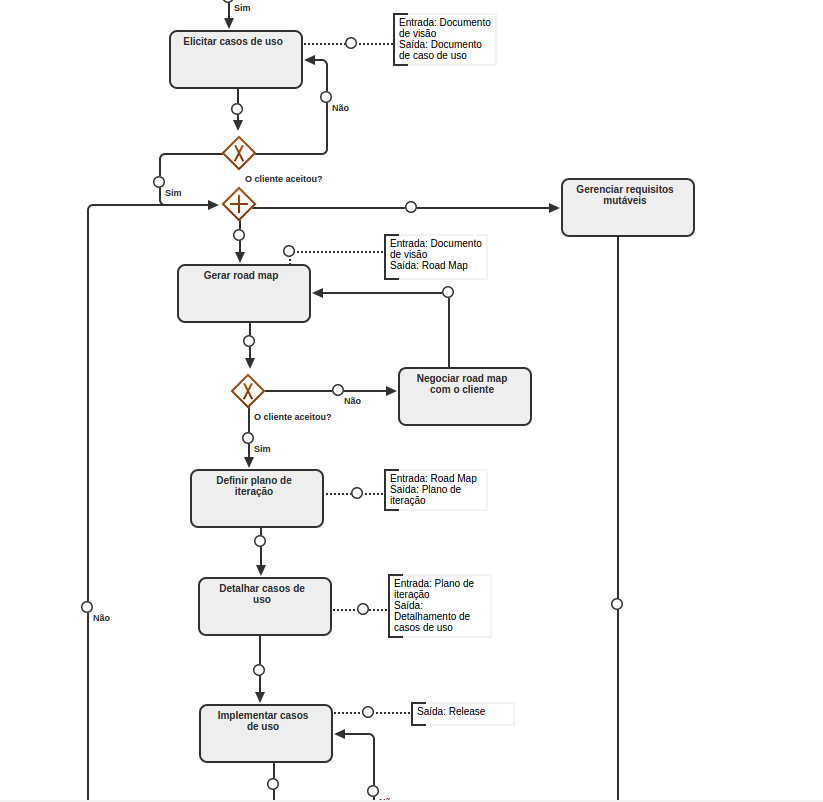
\includegraphics[width=0.8\textwidth]{imgModelagem/modelagem2}
	\caption{Modelagem Parte 2}
	\label{img:modelagem2}
\end{figure}

Após a implementação dos casos de uso da iteração, caso o cliente aceite, segue-se para a próxima iteração ou final do projeto, dependendo se existe ou não outros casos de uso a serem implantados, caso haja, o processo volta para as atividades de gerar o road map  e gerenciar requisitos mutáveis presentes na figura \ref{img:modelagem2}, assim como mostra a figura \ref{img:modelagem3}.

\begin{figure}[H]
	\centering
	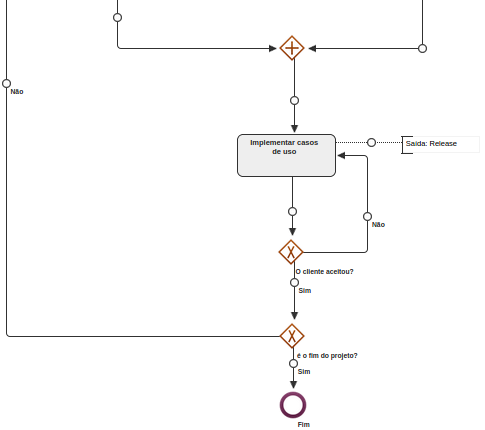
\includegraphics[width=0.8\textwidth]{imgModelagem/modelagem3}
	\caption{Modelagem Parte 3}
	\label{img:modelagem3}
\end{figure}
